\chapter{Evaluation}

- In this chapter, the Whisker testing utility is evaluated
- The focus of the evaluation lies in comparing the results of automated tests using Whisker to the results of manual assessment
- Additionally the results of using random input in conjunction to constraint-only tests is explored

- A collection of real Scratch programs from a student course is tested with four different test suites
- The first two test suites try to assess the projects as well as possible
- The second two test suites are used to find out if randomly generated user input can reasonably be used together with a constraint-only test suite

- Chapter outline

\section{Evaluation Method}
\subsection{Projects}
- From a students course
- Two groups, grade 6 and grade 7 $\rightarrow$ realistic for Whisker's purpose
- Multiple exercises to familiarize themselves with Scratch
- Build up to final, most complex, project
- Project has a clear description that stretches about half a DIN A4 page $\rightarrow$ well defined

=== Are these projects suitable for evaluating Whisker?
- Complexity on the higher end of what Whisker is supposed to be used for
- Game Over state makes it hard to assess other properties if the program goes game over because of a bug
    - E.g. one project would often go game over when an apple touches the borders on the sides
    - Well defined $\rightarrow$ tests can be written without looking at the projects (but often problematic, e.g. clones, inexact implementations)
- Students were not aware of the fact, that their projects would be subjected to automated assessment later
    - Students often deliberately changed their programs from the specification (e.g. different fall speeds, different messages)
    - In a real scenario (in which Whisker is used for grading) students would have the possibility to test their projects beforehand
    $\rightarrow$ see Chapter 2 - Advantages

\subsection{Excluded Projects}

\begin{table}
    \centering
    \scriptsize
    \begin{tabular}{ll}
        \toprule
        Project & Reason                                                                          \\
        \midrule
        \multicolumn{2}{l}{\textbf{Detected through the test report}}                             \\
        K6\_S12 & Deleted variable: time                                                          \\
        K6\_S17 & Renamed variable: "Punkte" to "Bunkte"                                          \\
        K7\_S24 & Deleted variable: time                                                          \\
        K7\_S27 & Renamed Sprite: "Bowl" to "Figur2"                                              \\[\medskipamount]

        \multicolumn{2}{l}{\textbf{Detected through zero statement coverage}}                     \\
        K6\_S01 & Starts on up key press instead of green flag                                    \\
        K6\_S06 & Wrong scratch project file (scored 30 points in manual rating but has no code)  \\
        K6\_S14 & Starts on space key press instead of green flag                                 \\[\medskipamount]

        \multicolumn{2}{l}{\textbf{Detected manually}}                                            \\
        K6\_S20 & Green flag has to be pressed twice to make it work properly                     \\
        K7\_S18 & Sprites have to be repositioned manually in the editor to make it work properly \\
        \bottomrule
    \end{tabular}
    \caption{Excluded Projects}
    \label{tab:excluded_projects}
\end{table}

\subsection{Tests}
- Normal + Constraint Tests
    - Deliberately control the bowl to win the game

- Normal Tests
    - Traditional testing approach: Each test checks one bit of the programs functionality
    - The program gets executed multiple times
    - Better for grading
    - Better for continuous development
    - Example of a normal test (or put it somewhere else?)

- Constraint Tests
    - Different approach: One test executes the program only once and checks defined constraints in the background
    - faster, but less accurate (show difference of average runtime)
    - not everything in this project can be tested in a single run
    - Better for quickly checking the program
    - Example of a constraint test (or put it somewhere else?)
    - Can be used with different sources of input (manual / simulated / random)
    - Instead of passing tests, passing constraints are measured
    - Tests with wrong sprite names are completely excluded in the evaluation

- Random Tests
    - Same constraints as the constraint tests
    - Random input instead of deliberately controlling the bowl
    - Random tests only make sense with constraints
        - defining single test cases would be difficult
        - execution would take a long time because most tests are skipped
    - Useful to test the stability of the program (like Android Monkey)
        - Although not on this particular project
    - This project is not well suited for random tests since random input will quickly result in a game over

Catch fruit with a bowl in order to not go game over and collect as many points as possible before the time is up.
\begin{table}
    \centering
    \scriptsize
    \begin{tabular}{lccc}
        \toprule
        Specification                                                                         & (1)    & (2)                   & (3)                   \\
        \midrule
        \textbf{Initialization} \\
        Timer starts at 30 seconds                                                            & \cmark & \xmark                & \xmark                \\
        Bowl starts at $X = 0$ / $Y = -145$                                                   & \cmark & \xmark                & \xmark                \\
        Fruits have a size of 50\%                                                            & \cmark & \cmark                & \cmark                \\[\medskipamount]
        \textbf{Bowl Movement} \\
        Bowl moves left/right when corresponding arrow key is pressed                         & \cmark & \cmark                & \cmark                \\
        Bowl can only move horizontally with a speed of 10                                    & \cmark & \cmark                & \cmark                \\[\medskipamount]
        \textbf{Fruit Falling} \\
        Apples fall down                                                                      & \cmark & \textasteriskcentered & \textasteriskcentered \\
        Apples fall in a straight line with a speed of -5                                     & \cmark & \cmark                & \cmark                \\
        Bananas fall down                                                                     & \cmark & \textasteriskcentered & \textasteriskcentered \\
        Bananas fall in a straight line with a speed of -7                                    & \cmark & \cmark                & \cmark                \\[\medskipamount]
        \textbf{Fruit Spawn} \\
        Apples spawn again at the top of the screen after touching the bowl                   & \cmark & \textasteriskcentered & \xmark                \\
        Apples spawn at random $X$ position                                                   & \cmark & \cmark                & \xmark                \\
        Apples spawn at $Y = 170$                                                             & \cmark & \cmark                & \xmark                \\
        Bananas spawn again at the top of the screen after touching the bowl                  & \cmark & \textasteriskcentered & \xmark                \\
        Bananas spawn at random $X$ position                                                  & \cmark & \cmark                & \xmark                \\
        Bananas spawn at $Y = 170$                                                            & \cmark & \cmark                & \xmark                \\
        Only one apple must fall down at a time                                               & \cmark & \cmark                & \xmark                \\
        Only one banana must fall down at a time                                              & \cmark & \cmark                & \xmark                \\
        Banana must wait for a second before falling down in the beginning                    & \cmark & \xmark                & \xmark                \\
        Banana must wait for a second before falling down after displaying the ''-8'' message & \cmark & \xmark                & \xmark                \\[\medskipamount]
        \textbf{Fruit Interaction} \\
        Apple gives 5 points when it touches the bowl                                         & \cmark & \cmark                & \cmark                \\
        Game over when the apple touches the ground                                           & \cmark & \textasteriskcentered & \cmark                \\
        Apple displays ''Game Over!'' message when it touches the ground                      & \cmark & \textasteriskcentered & \cmark                \\
        Banana gives 8 points when it touches the bowl                                        & \cmark & \cmark                & \cmark                \\
        Banana subtracts 8 points when it touches the ground                                  & \cmark & \cmark                & \cmark                \\
        Banana displays ''-8'' message when it touches the ground                             & \cmark & \cmark                & \cmark                \\[\medskipamount]
        \textbf{Timer} \\
        Timer ticks down                                                                      & \cmark & \cmark                & \cmark                \\
        Game is over when timer reaches 0                                                     & \cmark & \cmark                & \xmark                \\
        Bowl must display ''Ende!'' message when timer reaches 0                              & \cmark & \cmark                & \xmark                \\
        \bottomrule
    \end{tabular}
    \caption{Project specifications and their coverage by the test suites}
    \label{tab:specification}
\end{table}

\section{Evaluation Setup}

\begin{table}
    \centering
    \scriptsize \tt
    \begin{tabular}{ll}
        \toprule
        Whisker    & Whisker     1.0 \\
        Browser    & Chrome      70.0.3538.110 (64-Bit) \\
        JavaScript & V8          7.0.276.40 \\
        OS         & Windows 8.1 Version 6.3 (Build 9600) \\
        CPU        & Intel Core i5 4670 (4 x  3.40 GHz) \\
        GPU        & NVIDIA GeForce GTX 1080 \\
        RAM        & 8GB DDR3-1600 \\
        \bottomrule
    \end{tabular}
    \caption{Test setup}
    \label{tab:test_setup}
\end{table}


\section{Results}

\begin{figure}
    \centering
    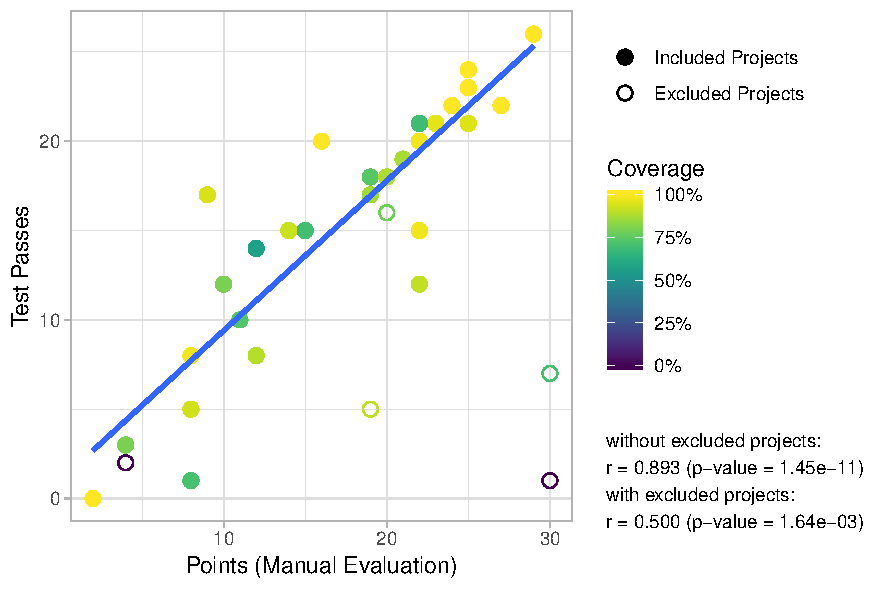
\includegraphics[width=.65\textwidth]{scatter-normal-1}
    \caption{Results of the normal test suite (1)}
    \label{fig:scatter_normal_1}
\end{figure}

\begin{figure}
    \centering
    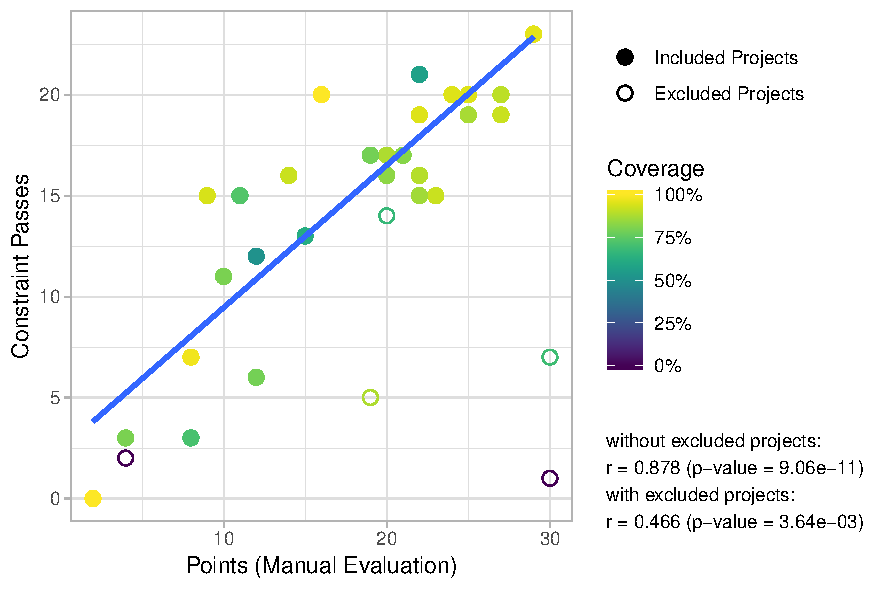
\includegraphics[width=.65\textwidth]{scatter-constraint-1}
    \caption{Results of the constraint test suite (2) \\ with deliberately simulated input}
    \label{fig:scatter_constraint_1}
\end{figure}

=== Normal Tests
- Manual analysis is used as ground truth

\section{Threats to validity}
- Students often deliberately changed their programs from the specification (e.g. different fall speeds)
    - Tests were adjusted to allow a little more than the specification (e.g. different message)

- For each tests suite, many / all projects were executed in a row
    - Could have a performance impact (?), but Scratch doesn't need a lot of resources
    - If anything, it could have a negative impact on the results, but results are very positive
